\documentclass[titlepage]{article}
\usepackage{babel}
\usepackage{amsmath}
\usepackage{amssymb}
\usepackage{amsthm}
\usepackage{stmaryrd} %ligtning

\usepackage{tabto} %tabulator mit \tab
\usepackage{tikz}
\usetikzlibrary{automata, arrows.meta, positioning, shadows, shapes.geometric} % automaten zeichnen
\usepackage[utf8]{inputenc}
\pagestyle{plain}
\pagenumbering{arabic}
\renewcommand{\arraystretch}{1.3} %vertikaler abstand von tabellen
\usepackage[left=20mm, right=15mm, top=25mm, bottom=7mm, paper=a4paper]{geometry}

\renewcommand{\contentsname}{Inhaltsverzeichnis}
\renewcommand{\]}{\right]}
\renewcommand{\[}{\left[}
\renewcommand{\)}{\right)}
\renewcommand{\(}{\left(}
\renewcommand{\|}{\;|\;}
\newcommand{\n}{\newline}
\renewcommand{\l}{\linebreak}



\begin{document}\begingroup\let\clearpage\relax
	%header
	\begin{center}
	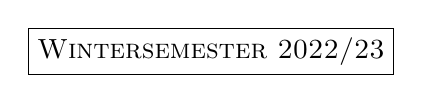
\begin{tikzpicture}
		\draw (0,0) node[draw, rectangle]{\textsc{Wintersemester 2022/23}};
	\end{tikzpicture}
	\hrulefill\\
	\begin{center}
		\LARGE\textsc{Automaten und Berechenbarkeit - Übung 04} \normalsize\\
	\end{center}
	\hrulefill
	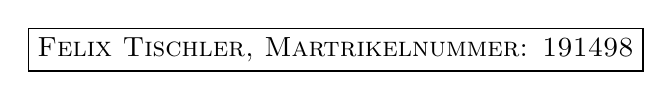
\begin{tikzpicture}
		\draw (0,0) node[draw, rectangle]{\textsc{Felix Tischler, Martrikelnummer: 191498}};
	\end{tikzpicture}
	\date{\today}
\end{center}
	
	%task one
	\section*{Aufgabe 1}
		\include{t1.tex}
		
	\section*{Aufgabe 2}
		\newcommand{\nc[4]}{#2&#3&#4\\\hline}
\begin{center}
	$M=(\{0,1\},\{0,0_1,0_2,0_3,1,2,2_1,2_2,2_3,2_4,2_5\},\delta,\{0_1\},\{0_2,1,2,2_1,2_4\})$
	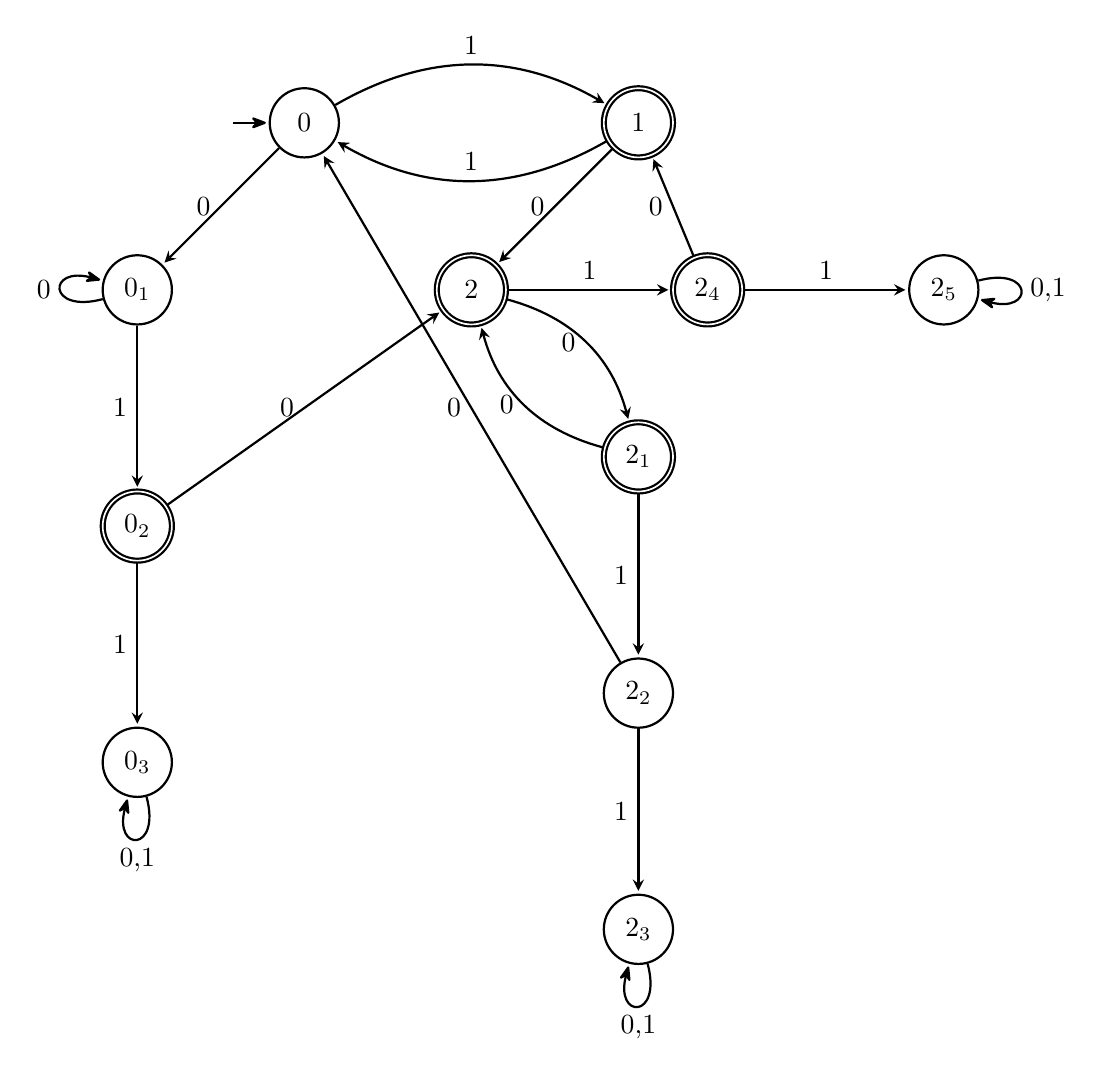
\begin{tikzpicture}[shorten >=1pt,node distance=3cm,on grid,>={Stealth[round]},thick]
		
		\node (q2) 
			[state, accepting] {2};
			\node (q21) 
				[state, accepting, below right of = q2] {$2_1$};
			\node (q22) 
				[state, below of = q21] {$2_2$};
			\node (q23) 
				[state, below of = q22] {$2_3$};
				
			\node (q24) 
				[state, accepting, right of = q2] {$2_4$};
			\node (q25) 
				[state, right of = q24] {$2_5$};
			
			
		\node (q0) 
			[state, initial, initial text = {}, above left of = q2] {0};
			\node (q01) 
				[state, below left of = q0] {$0_1$};
			\node (q02) 
				[state, accepting, below of = q01] {$0_2$};
			\node (q03) 
				[state, below of = q02] {$0_3$};
			
			
		\node (q1) 
			[state, accepting, above right of = q2] {1};
			
		
		
		\path [-stealth, thick]
		%(q0) edge [loop above] node [above] {$0$} (q0)
		(q0) edge [bend left] node [above] {1} (q1)
		(q0) edge node [left] {0} (q01)
		(q01) edge node [left] {1} (q02)
		(q02) edge node [left] {1} (q03)
		(q03) edge [loop below] node [below] {0,1} (q03)
		
		(q1) edge [bend left] node [above] {1} (q0)
		(q1) edge node [left] {0} (q2)
		
		(q2) edge [bend left] node [left] {0} (q21)
		(q21) edge [bend left] node [left] {0} (q2)
		(q21) edge node [left] {1} (q22)
		(q22) edge node [left] {1} (q23)
		(q22) edge node [left] {0} (q0)
		
		(q2) edge node [above] {1} (q24)
		(q24) edge node [above] {1} (q25)
		
		(q01) edge [loop left] node [left] {0} (q01)
		(q23) edge [loop below] node [below] {0,1} (q23)
		(q24) edge node [left] {0} (q1)
		(q25) edge [loop right] node [right] {0,1} (q25)
		(q02) edge node [left] {0} (q2)
		;
	\end{tikzpicture}
	
	$\delta:$
	\begin{table}[h]
		\centering
		\begin{tabular}{|c|c|c|}
			\hline
			Zustand & $0$ & $1$ \\
			\hline\hline
			\nc{$0$}{$0_1$}{$1$}
			\nc{$0_1$}{$0_1$}{$0_2$}
			\nc{$0_2$}{$2$}{$0_3$}
			\nc{$0_3$}{$0_3$}{$0_3$}
			\nc{$1$}{$2$}{$0$}
			\nc{$2$}{$2_1$}{$2_4$}
			\nc{$2_1$}{$2$}{$2_2$}
			\nc{$2_2$}{$0$}{$2_3$}
			\nc{$2_3$}{$2_3$}{$2_3$}
			\nc{$2_4$}{$1$}{$2_5$}
			\nc{$2_5$}{$2_5$}{$2_5$}
		\end{tabular}
	\end{table}
\end{center}
Der Automat ist folgendermaßen entstanden: Ich habe den Automaten der letzten Übungsserie genommen in dem beschrieben wird wann eine binär Zahl durch 3 teilbar ist:
\begin{center}
	$M_2=(\{0,1\},\{\equiv_3=0,\equiv_3=1,\equiv_3=2\},\delta_2,\{\equiv_3=0\},\{\equiv_3=0\})$\\
	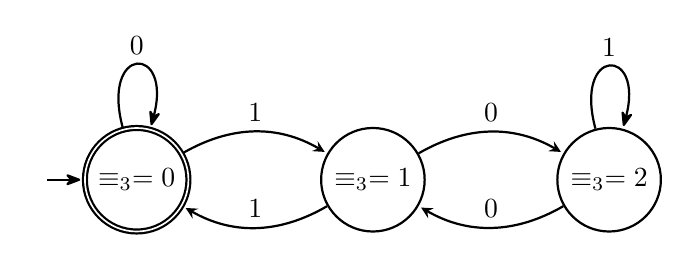
\begin{tikzpicture}[shorten >=1pt,node distance=3cm,on grid,>={Stealth[round]},thick]
		
		\node (q0) [state,initial, accepting, initial text = {}] {$\equiv_3=0$};
		\node (q1) [state, right of = q0] {$\equiv_3=1$};
		\node (q2) [state, right of = q1] {$\equiv_3=2$};
		
		\path [-stealth, thick]
		(q0) edge [loop above] node [above] {$0$} (q0)
		(q0) edge [bend left] node [above] {$1$} (q1)
		(q1) edge [bend left] node [above] {$1$} (q0)
		(q1) edge [bend left] node [above] {$0$} (q2)
		(q2) edge [bend left] node [above] {$0$} (q1)
		(q2) edge [loop above] node [above] {$1$} (q2);
		
	\end{tikzpicture}
	
	$\delta_2:$
	\begin{table}[h]
		\centering
		\begin{tabular}{|c|c|c|}
			\hline
			Zustand & $0$ & $1$ \\
			\hline\hline
			$\emptyset$&$\emptyset$&$\emptyset$\\
			\hline
			$\equiv_3=0$&\nm[$\equiv_3=0$]&\nm[$\equiv_3=1$]\\
			\hline
			$\equiv_3=1$&\nm[$\equiv_3=2$]&\nm[$\equiv_3=0$]\\
			\hline
			$\equiv_3=1$&\nm[$\equiv_3=1]$&\nm[$\equiv_3=2$]\\
			\hline
		\end{tabular}
	\end{table}
\end{center}
Von hier aus habe ich dann alle Fälle betrachtet in denen eine $0$ gelesen wird und habe diese dann zu einem dedizierten Zustand weitergeleitet. In jedem dieser Fälle habe ich dann betrachtet wie sich sowohl die Nicht-Teilbarkeit durch 3 verhält, als auch ob ein neuer Zustand benötigt wird um das Teilwort $011$ zu kapseln. Dieser Automat kann prinzipiell jedes Wort lesen. Wenn jedoch eine Sequenz $011$ auftritt, egal wo man sich vorher befunden hat, so  endet man in $0_3\lor2_3\lor2_5$. Somit ist wenn dieses Teilwort aufgetreten ist es nicht mehr möglich akzeptiert zu werden. In allen anderen fällen ist es möglich ein Wort zu lesen, dass akzeptiert wird, hierfür muss jedoch die Nicht-Teilbarkeit durch 3 gegeben sein. Dieses habe ich mittels dem Automaten der Übungsserie 4 abgeleitet. Jeder Zustand im Automaten besitzt neben der Information welche Zahlen vor ihm gelesen wurden auch die Information ob er durch 3 Teilbar ist oder nicht. Diese Informationen verteilen sich wie folgt: $0,0_1,2_2$ sind durch 3 teilbar. $1,0_2,2_1$ sind durch 3 Rest 1 teilbar und somit zu akzeptieren. Und $2,2_4$ sind durch 3 Rest 2 teilbar und folglich auch zu akzeptieren. 
	
\endgroup\end{document}